\begin{frame}
  \frametitle{Il teorema di Wolff-Denjoy}
  \only<1-5>{Sia $\mathbb{D}$ il disco unitario in $\mathbb{C}$.\pause
  \begin{block}{Teorema (Wolff-Denjoy, 1926)}
    \begin{itshape}
      Sia $f:\mathbb{D} \longrightarrow \mathbb{D}$ una funzione olomorfa. \pause Allora vale esattamente una delle seguenti affermazioni:\pause
      \begin{itemize}
        \item la funzione $f$ ha un punto fisso nel disco; \pause oppure,
        \item esiste un unico punto del bordo del disco tale che la successione delle iterate di $f$ converge, uniformemente sui compatti, a quel punto.
      \end{itemize}
    \end{itshape}
  \end{block}}
  \only<6->{
    - Abate, 1991: generalizzazione in più variabili al caso di domini limitati, strettamente pseudoconvessi e taut.\\ \setcounter{beamerpauses}{6}\pause
    Cosa cambia: non più un punto fisso, ma orbite relativamente compatte. In questo caso, la dinamica è nota;\\ \pause
    - Abate, Heinzner, 1992: esistono esempi con orbite relativamente compatte, ma senza punti fissi; \\ \pause
    - Balogh, Bonk, 2000: i domini limitati e strettamente pseudoconvessi, dotati di un'opportuna distanza, sono Gromov-iperbolici.
  }
\end{frame}

\begin{frame}[t]
  \frametitle{La condizione di visibilità}
  \only<1-4>{
    \begin{defn}
      Sia $X$ una varietà complessa; la \textit{pseudometrica di Kobayashi} su $X$ è
      \begin{equation*}\begin{split}
          K_X(x;Z)=\inf\{&|v| \mid v \in \mathbb{C}, \text{ esiste }f \in \text{Hol}(\mathbb{D},X) \\
          &\text{ tale che } f(0)=x, \diff_0 f(v)=Z\}
      \end{split}\end{equation*}
      per ogni $x \in X$ e $Z \in T_xX$.\pause
      
      Se $X$ è connessa, la \textit{pseudodistanza di Kobayashi} è $k_X$, la forma integrata di $K_X$.
    \end{defn}
  }

  \only<3-4>{
    Le funzioni olomorfe sono semicontrazioni sia rispetto a $K_X$ che rispetto a $k_X$.
  }

  \only<4>{
    Se $k_X$ è una distanza, induce la topologia di varietà; in tal caso, $X$ è detta \textit{Kobayashi-iperbolica}.
  }
  \only<5-8>{
    \begin{defn}
      Sia $X$ una varietà complessa e connessa; fissiamo due costanti $\lambda \ge 1$ e $\kappa \ge 0$. Sia $I\subseteq \mathbb{R}$ un intervallo; \setcounter{beamerpauses}{5}\pause una curva $\sigma:I \longrightarrow X$ è detta una \textit{$(\lambda,\kappa)$-simil-geodetica} se:\pause
    \begin{enumerate}
        \item per ogni $s,t \in I$ si ha
        \begin{equation*}
            \frac{1}{\lambda}|t-s|-\kappa \le k_X\big(\sigma(s),\sigma(t)\big)\le\lambda|t-s|+\kappa;
        \end{equation*}\pause
        \item $\sigma$ è assolutamente continua (quindi $\sigma'(t)$ esiste per quasi ogni $t \in I$) e per quasi ogni $t \in I$ si ha
        \begin{equation*}
            K_X\big(\sigma(t);\sigma'(t)\big) \le \lambda.
        \end{equation*}
    \end{enumerate}
    \end{defn}
  }
  \only<9-12>{
    \begin{defn}
      Sia $X$ una sottovarietà complessa e connessa di una varietà complessa $Y$, e fissiamo $\lambda \ge 1$ e $\kappa \ge 0$. \setcounter{beamerpauses}{9}\pause Diciamo che $X$ è \textit{$(\lambda,\kappa)$-visibile} se:\pause
      \begin{enumerate}
          \item ogni due punti distinti di $X$ possono essere collegati da una $(\lambda,\kappa)$-simil-geodetica;\pause
          \item per ogni coppia di punti $p,q\in\partial_YX$ con $p\not=q$, esistono in $\overline{X}$ due intorni $V$ e $W$, di $p$ e $q$ rispettivamente, con chiusura disgiunta, e un compatto $K$ di $X$ tali che  ogni $(\lambda,\kappa)$-simil-geodetica in $X$ che collega un punto di $V$ a un punto di $W$ interseca $K$.
      \end{enumerate}
      \begin{center}
        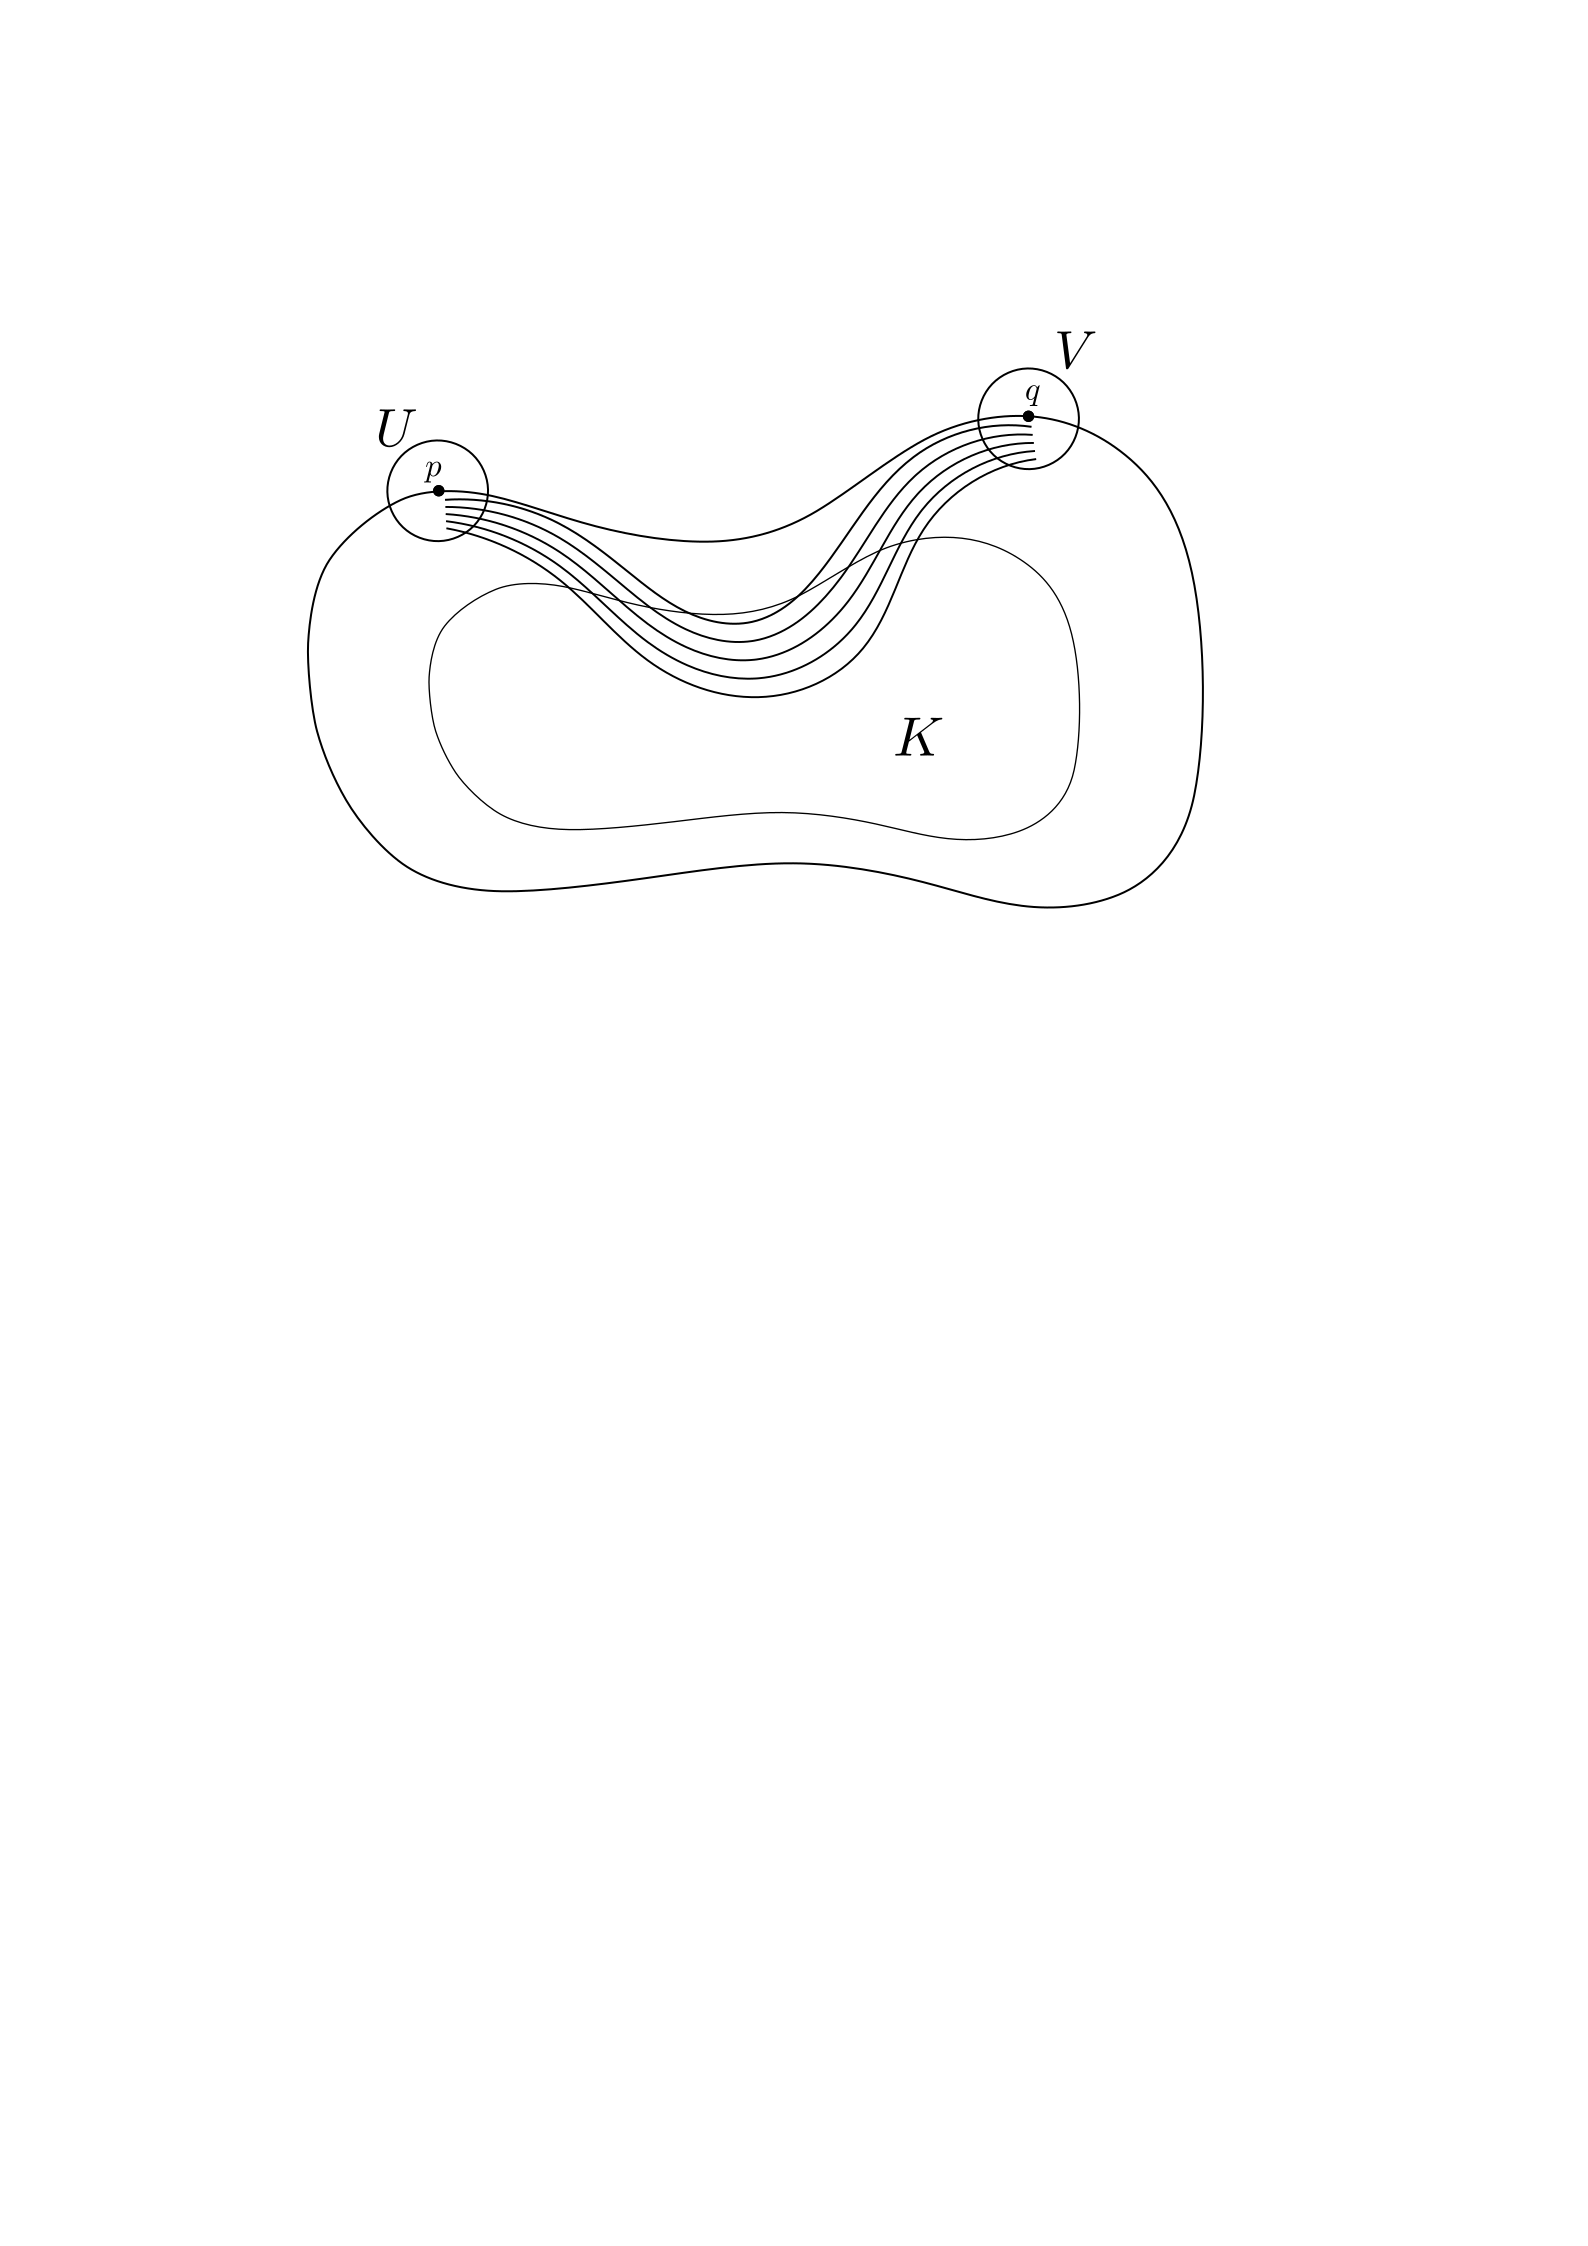
\includegraphics[width=0.60\textwidth, trim=0 17.5cm 0 5cm]{vis.png}
      \end{center}
  \end{defn}
  }
  \only<13-17>{
    Caso escluso: le simil-geodetiche da $U$ a $V$ fuggono dal compatto $K$.
  }
  \only<13>{
    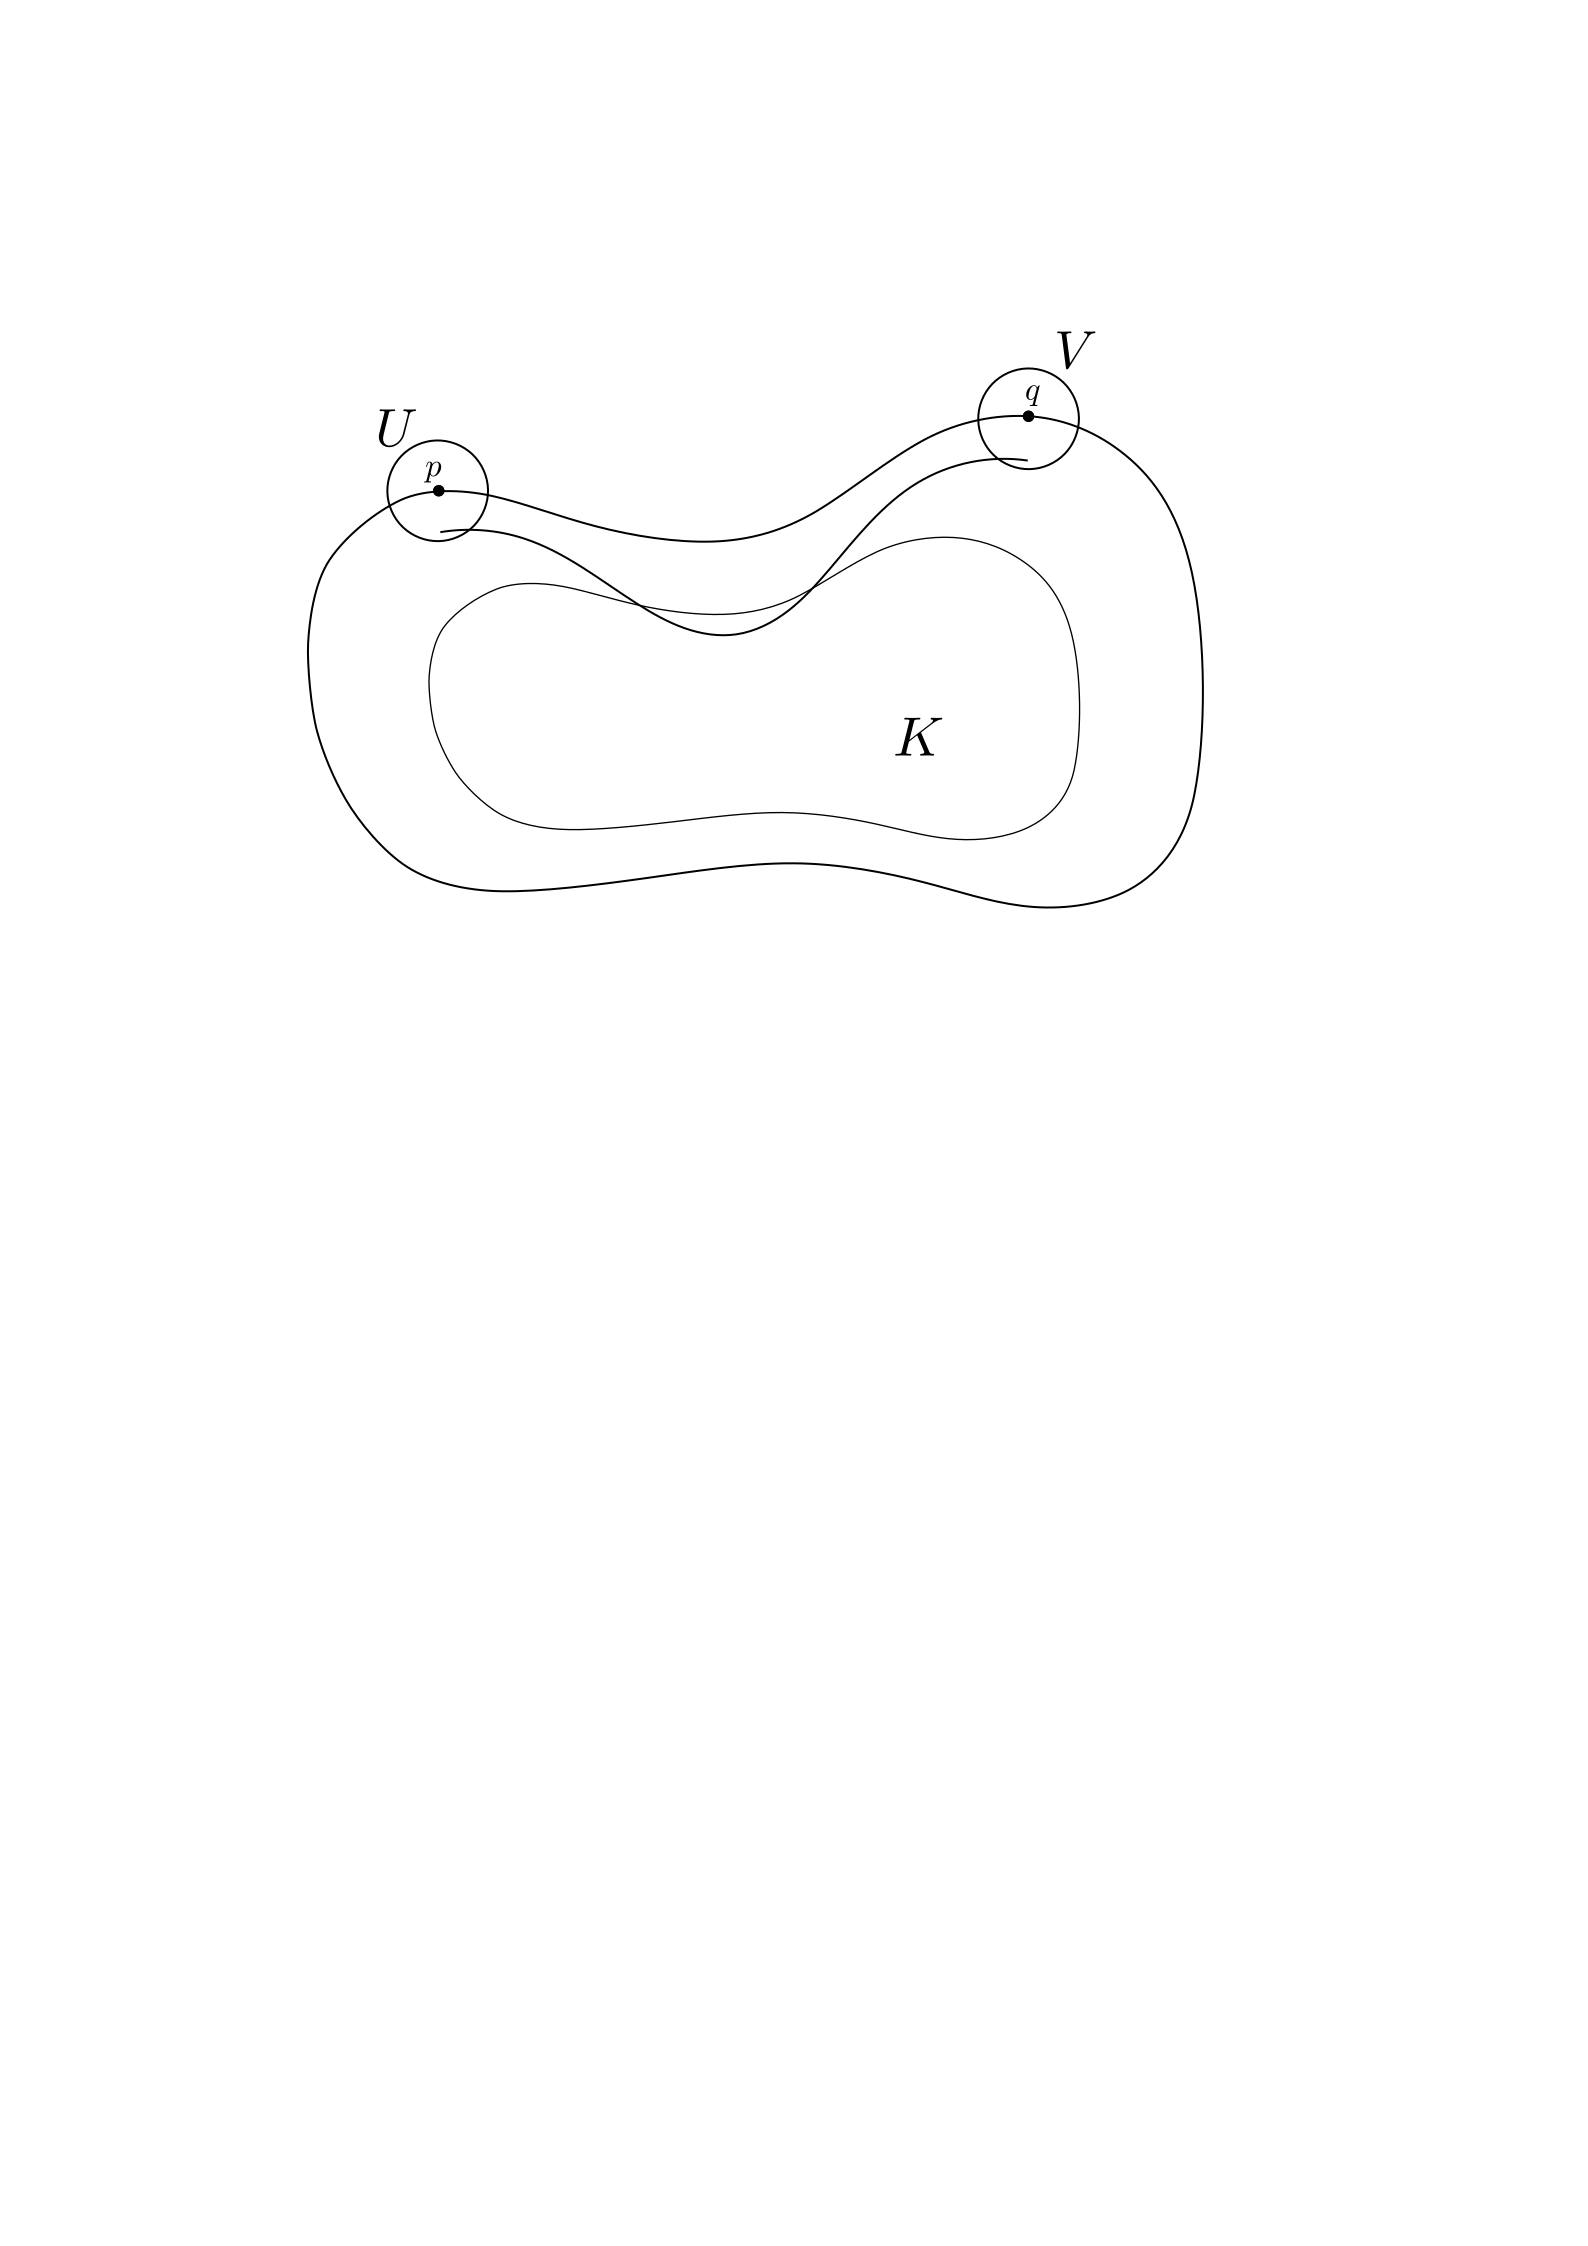
\includegraphics[width=1.05\textwidth, trim=0 18cm 0 3cm]{nonvis1.png}
  }
  \only<14>{
    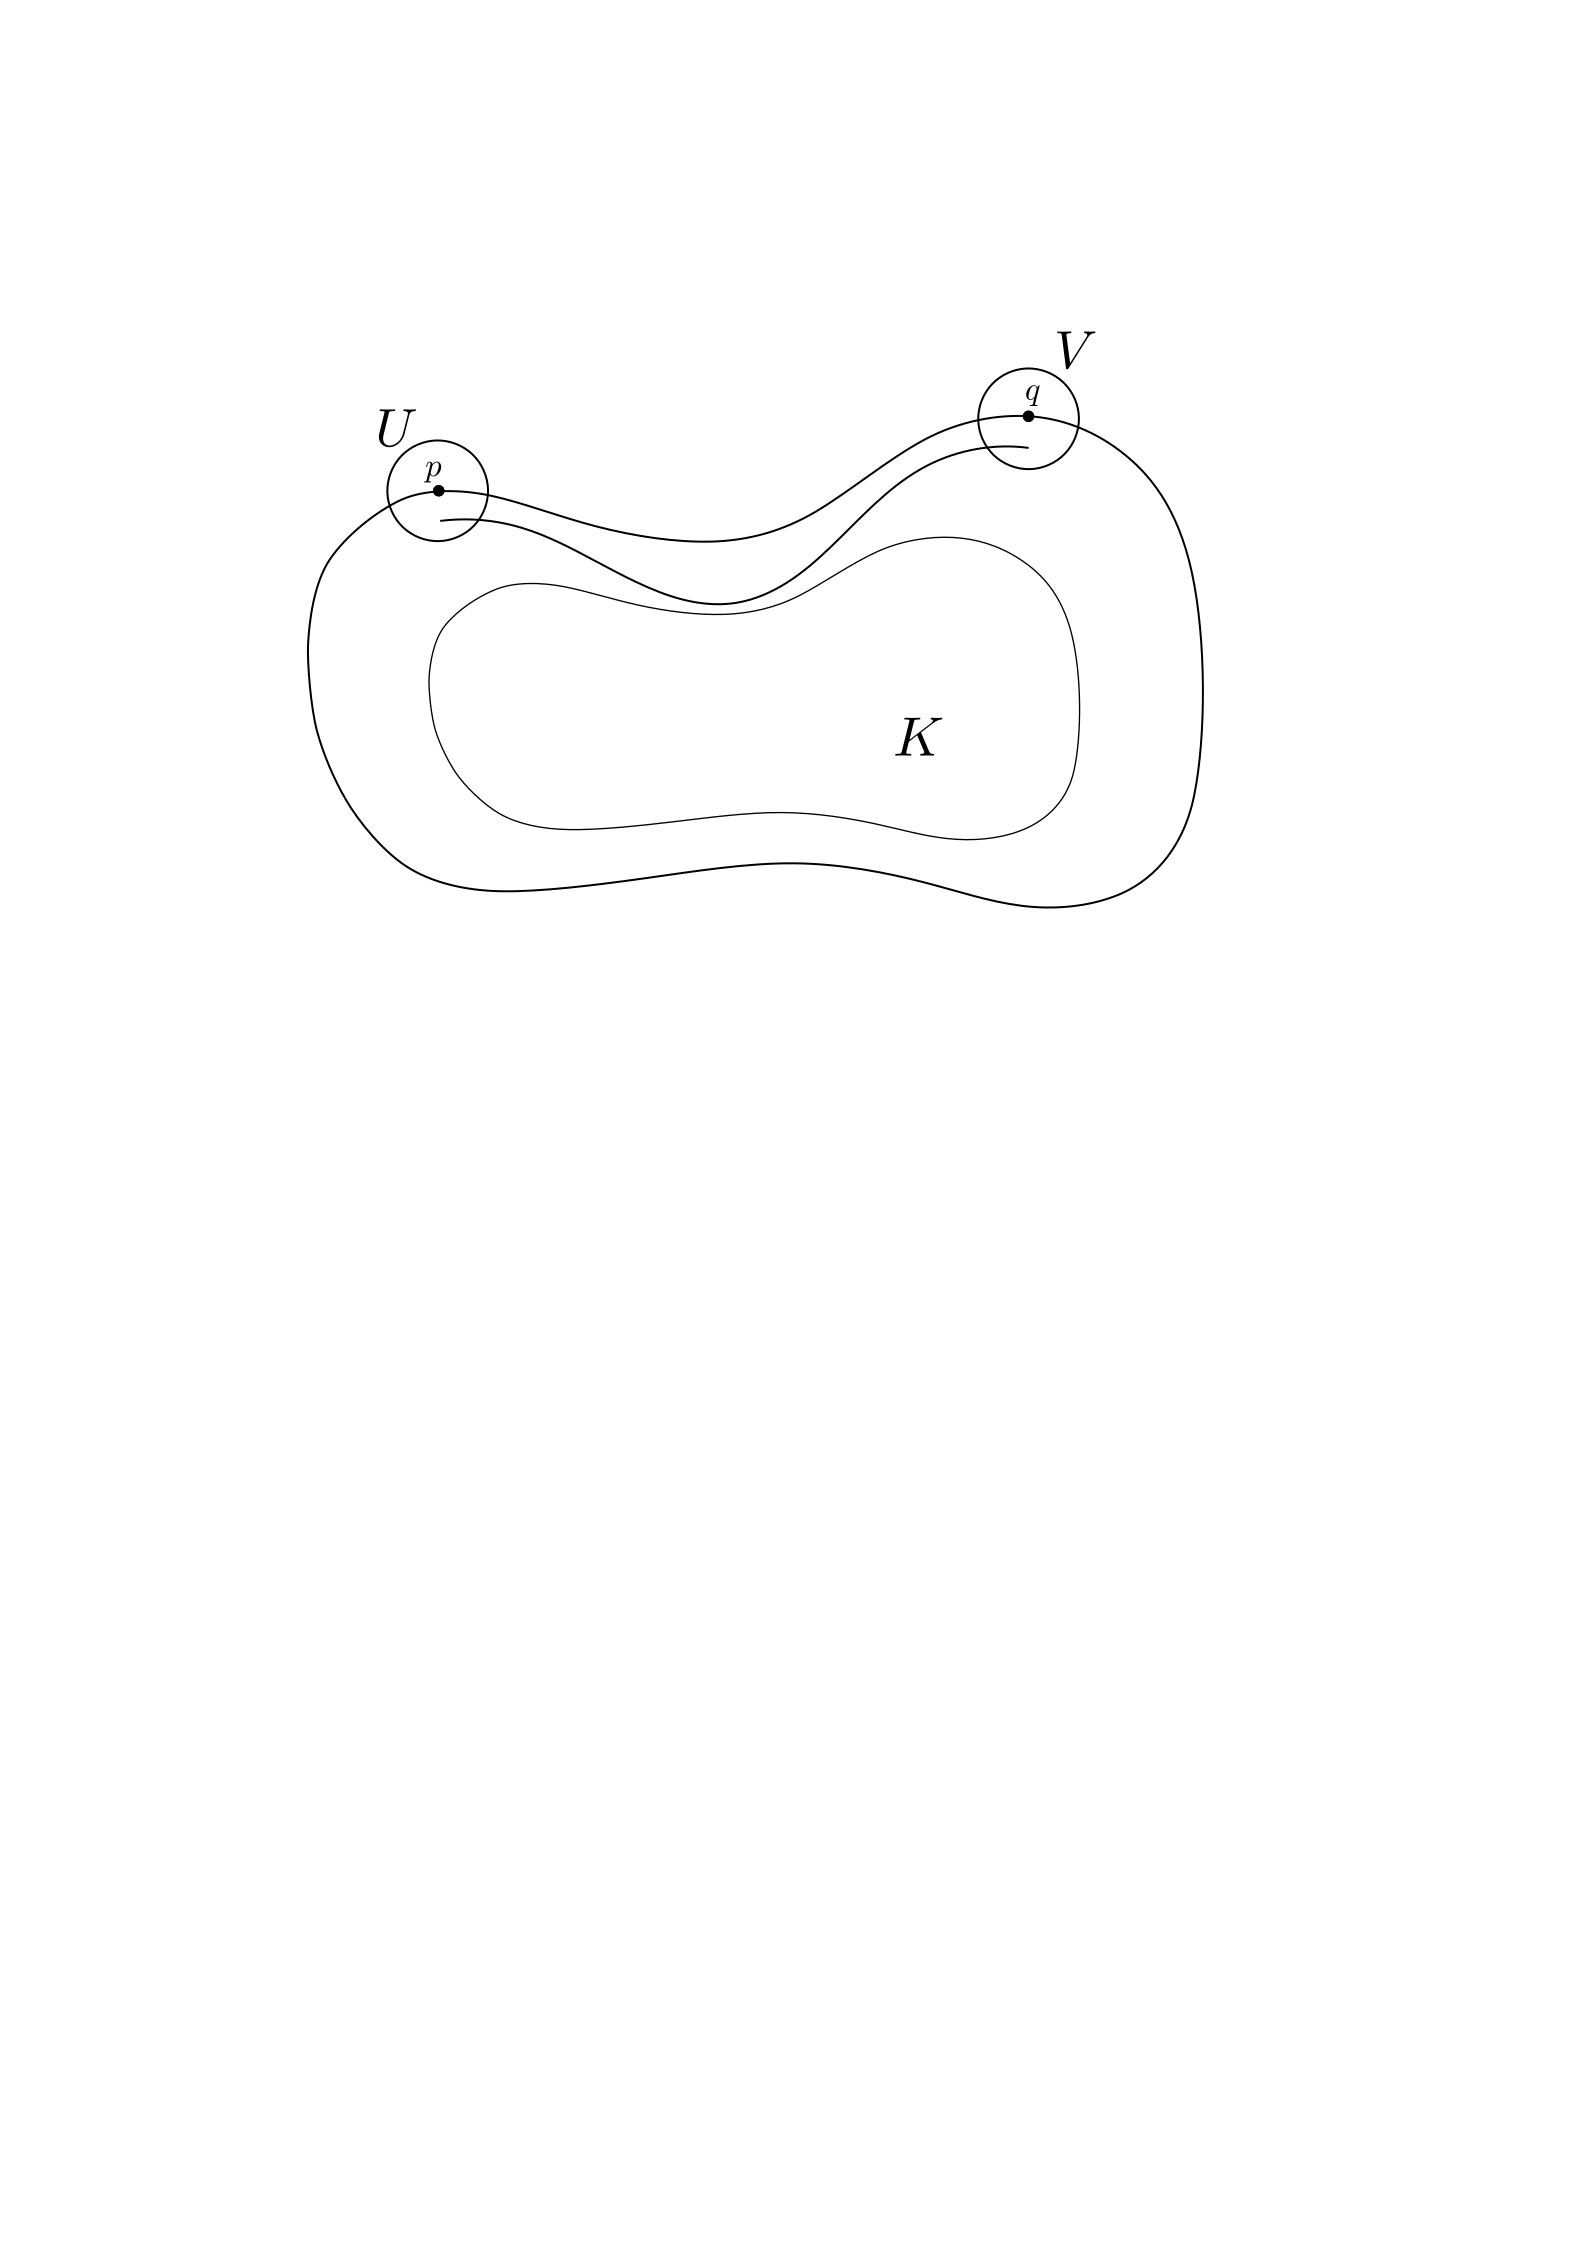
\includegraphics[width=1.05\textwidth, trim=0 18cm 0 3cm]{nonvis2.png}
  }
  \only<15>{
    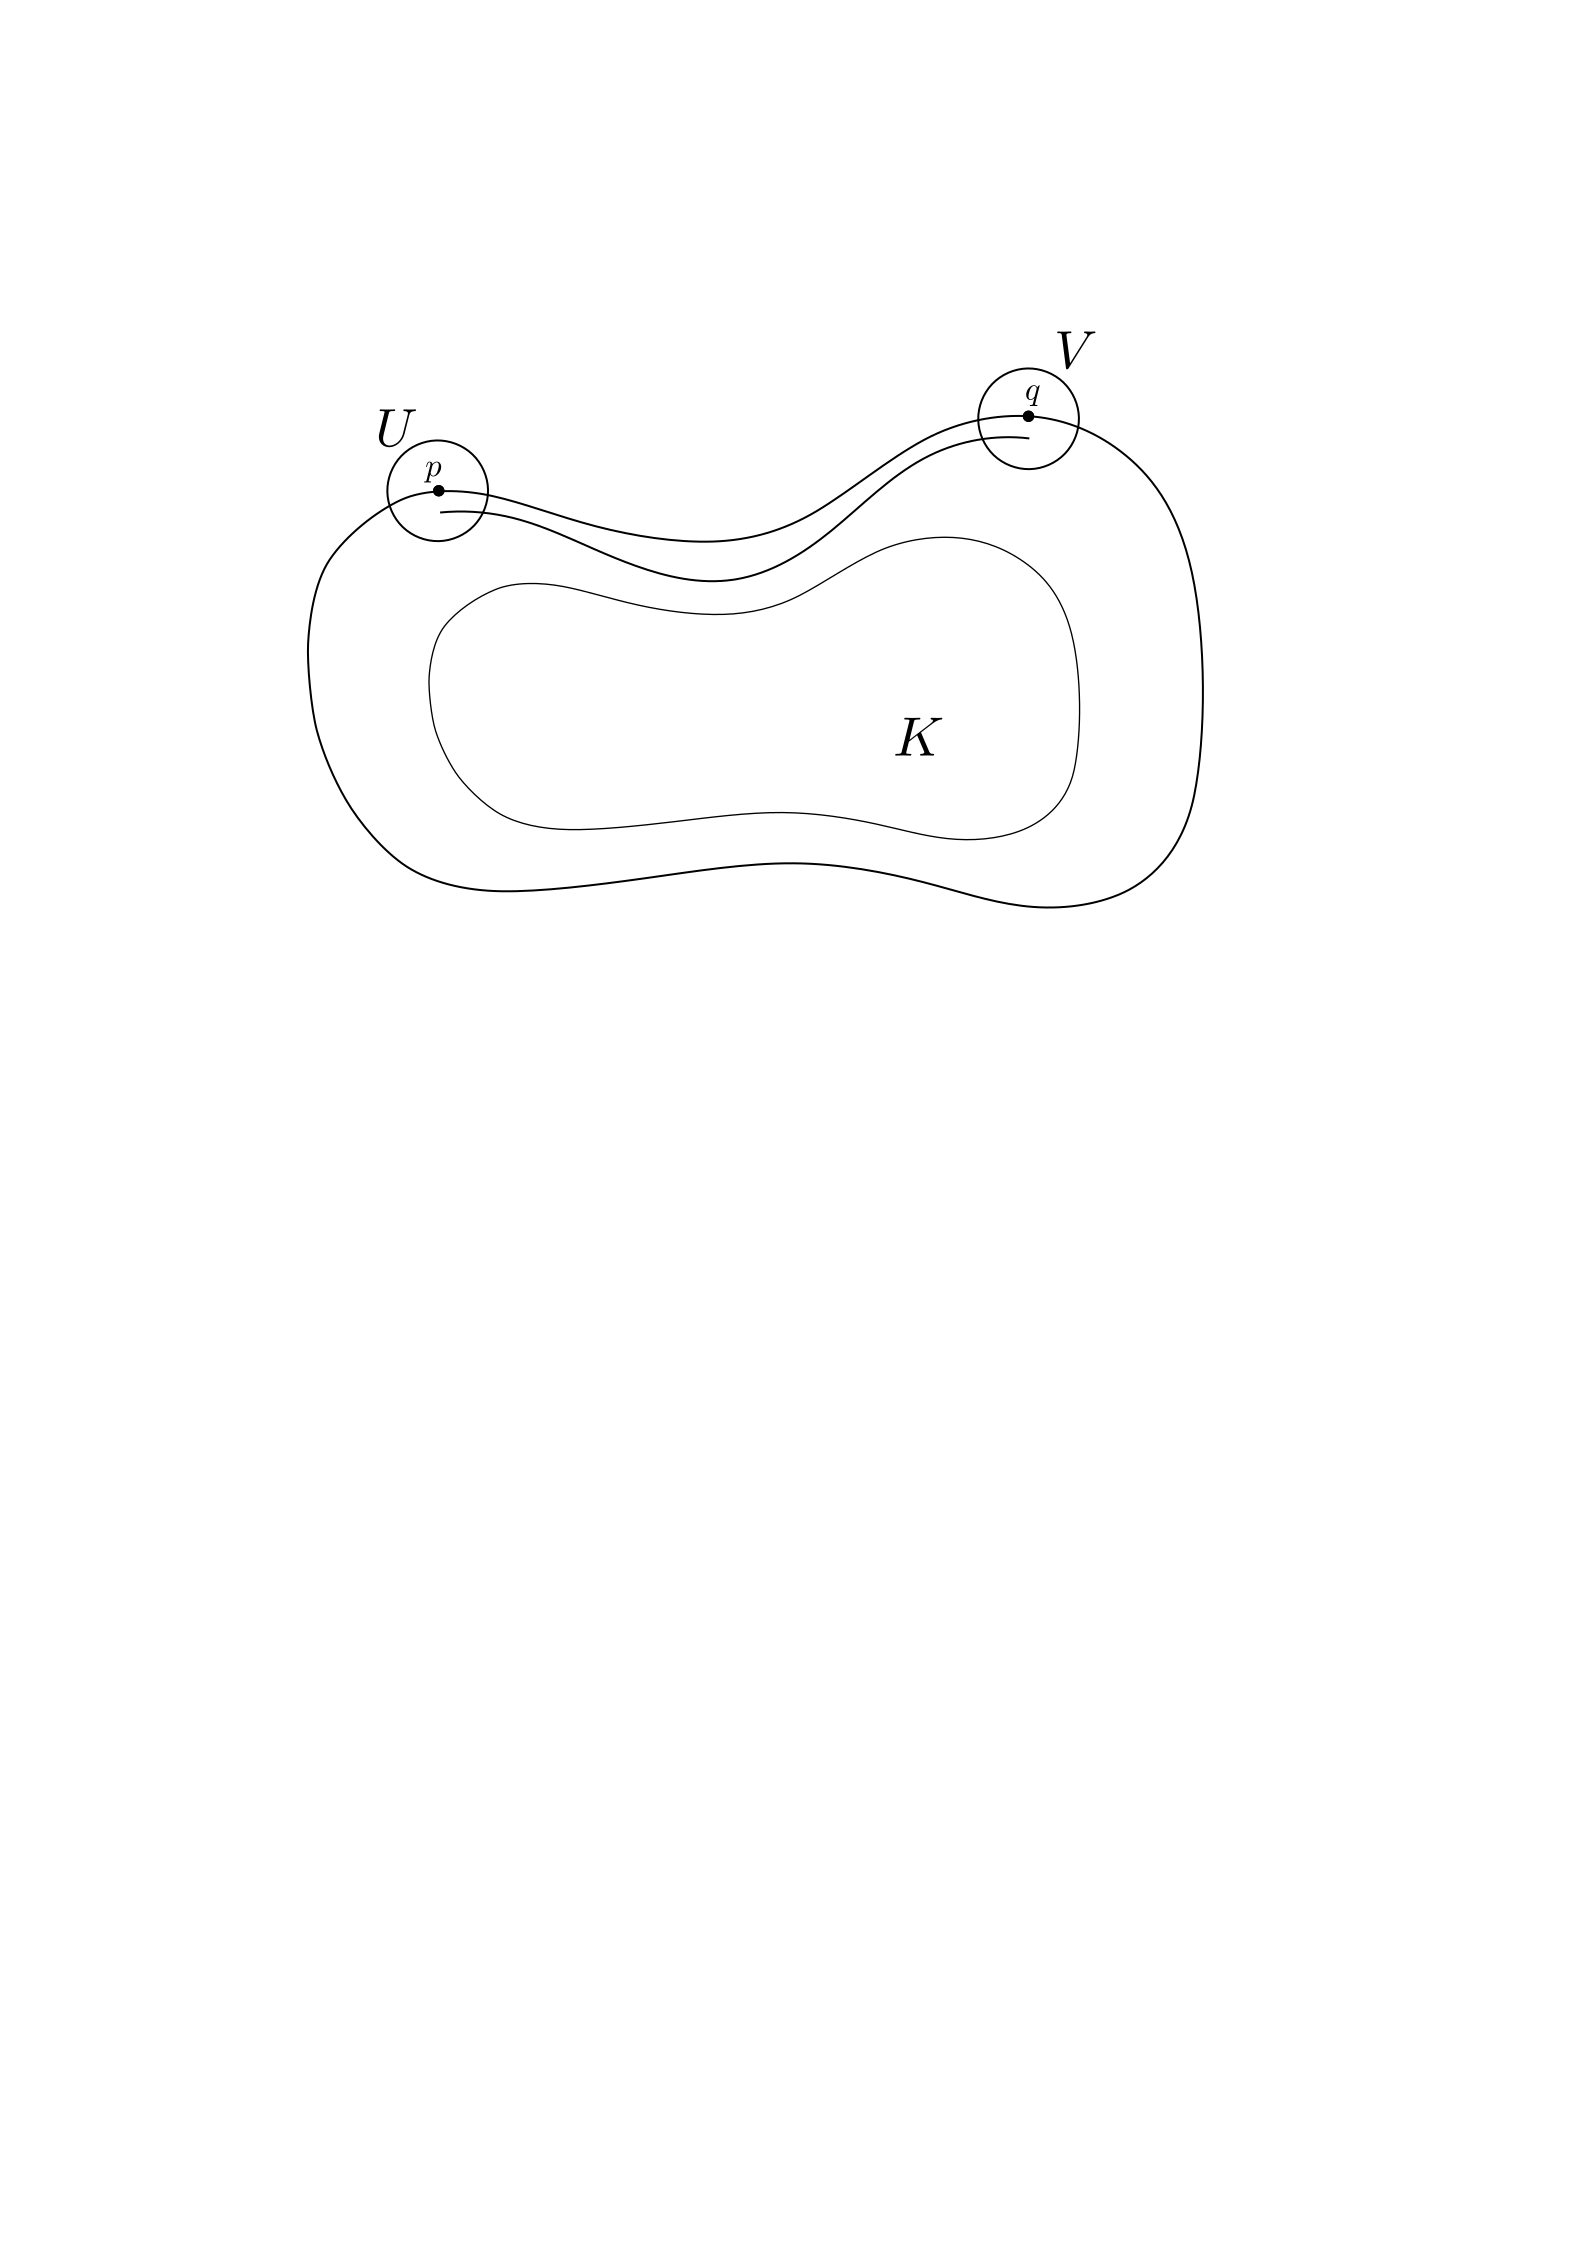
\includegraphics[width=1.05\textwidth, trim=0 18cm 0 3cm]{nonvis3.png}
  }
  \only<16>{
    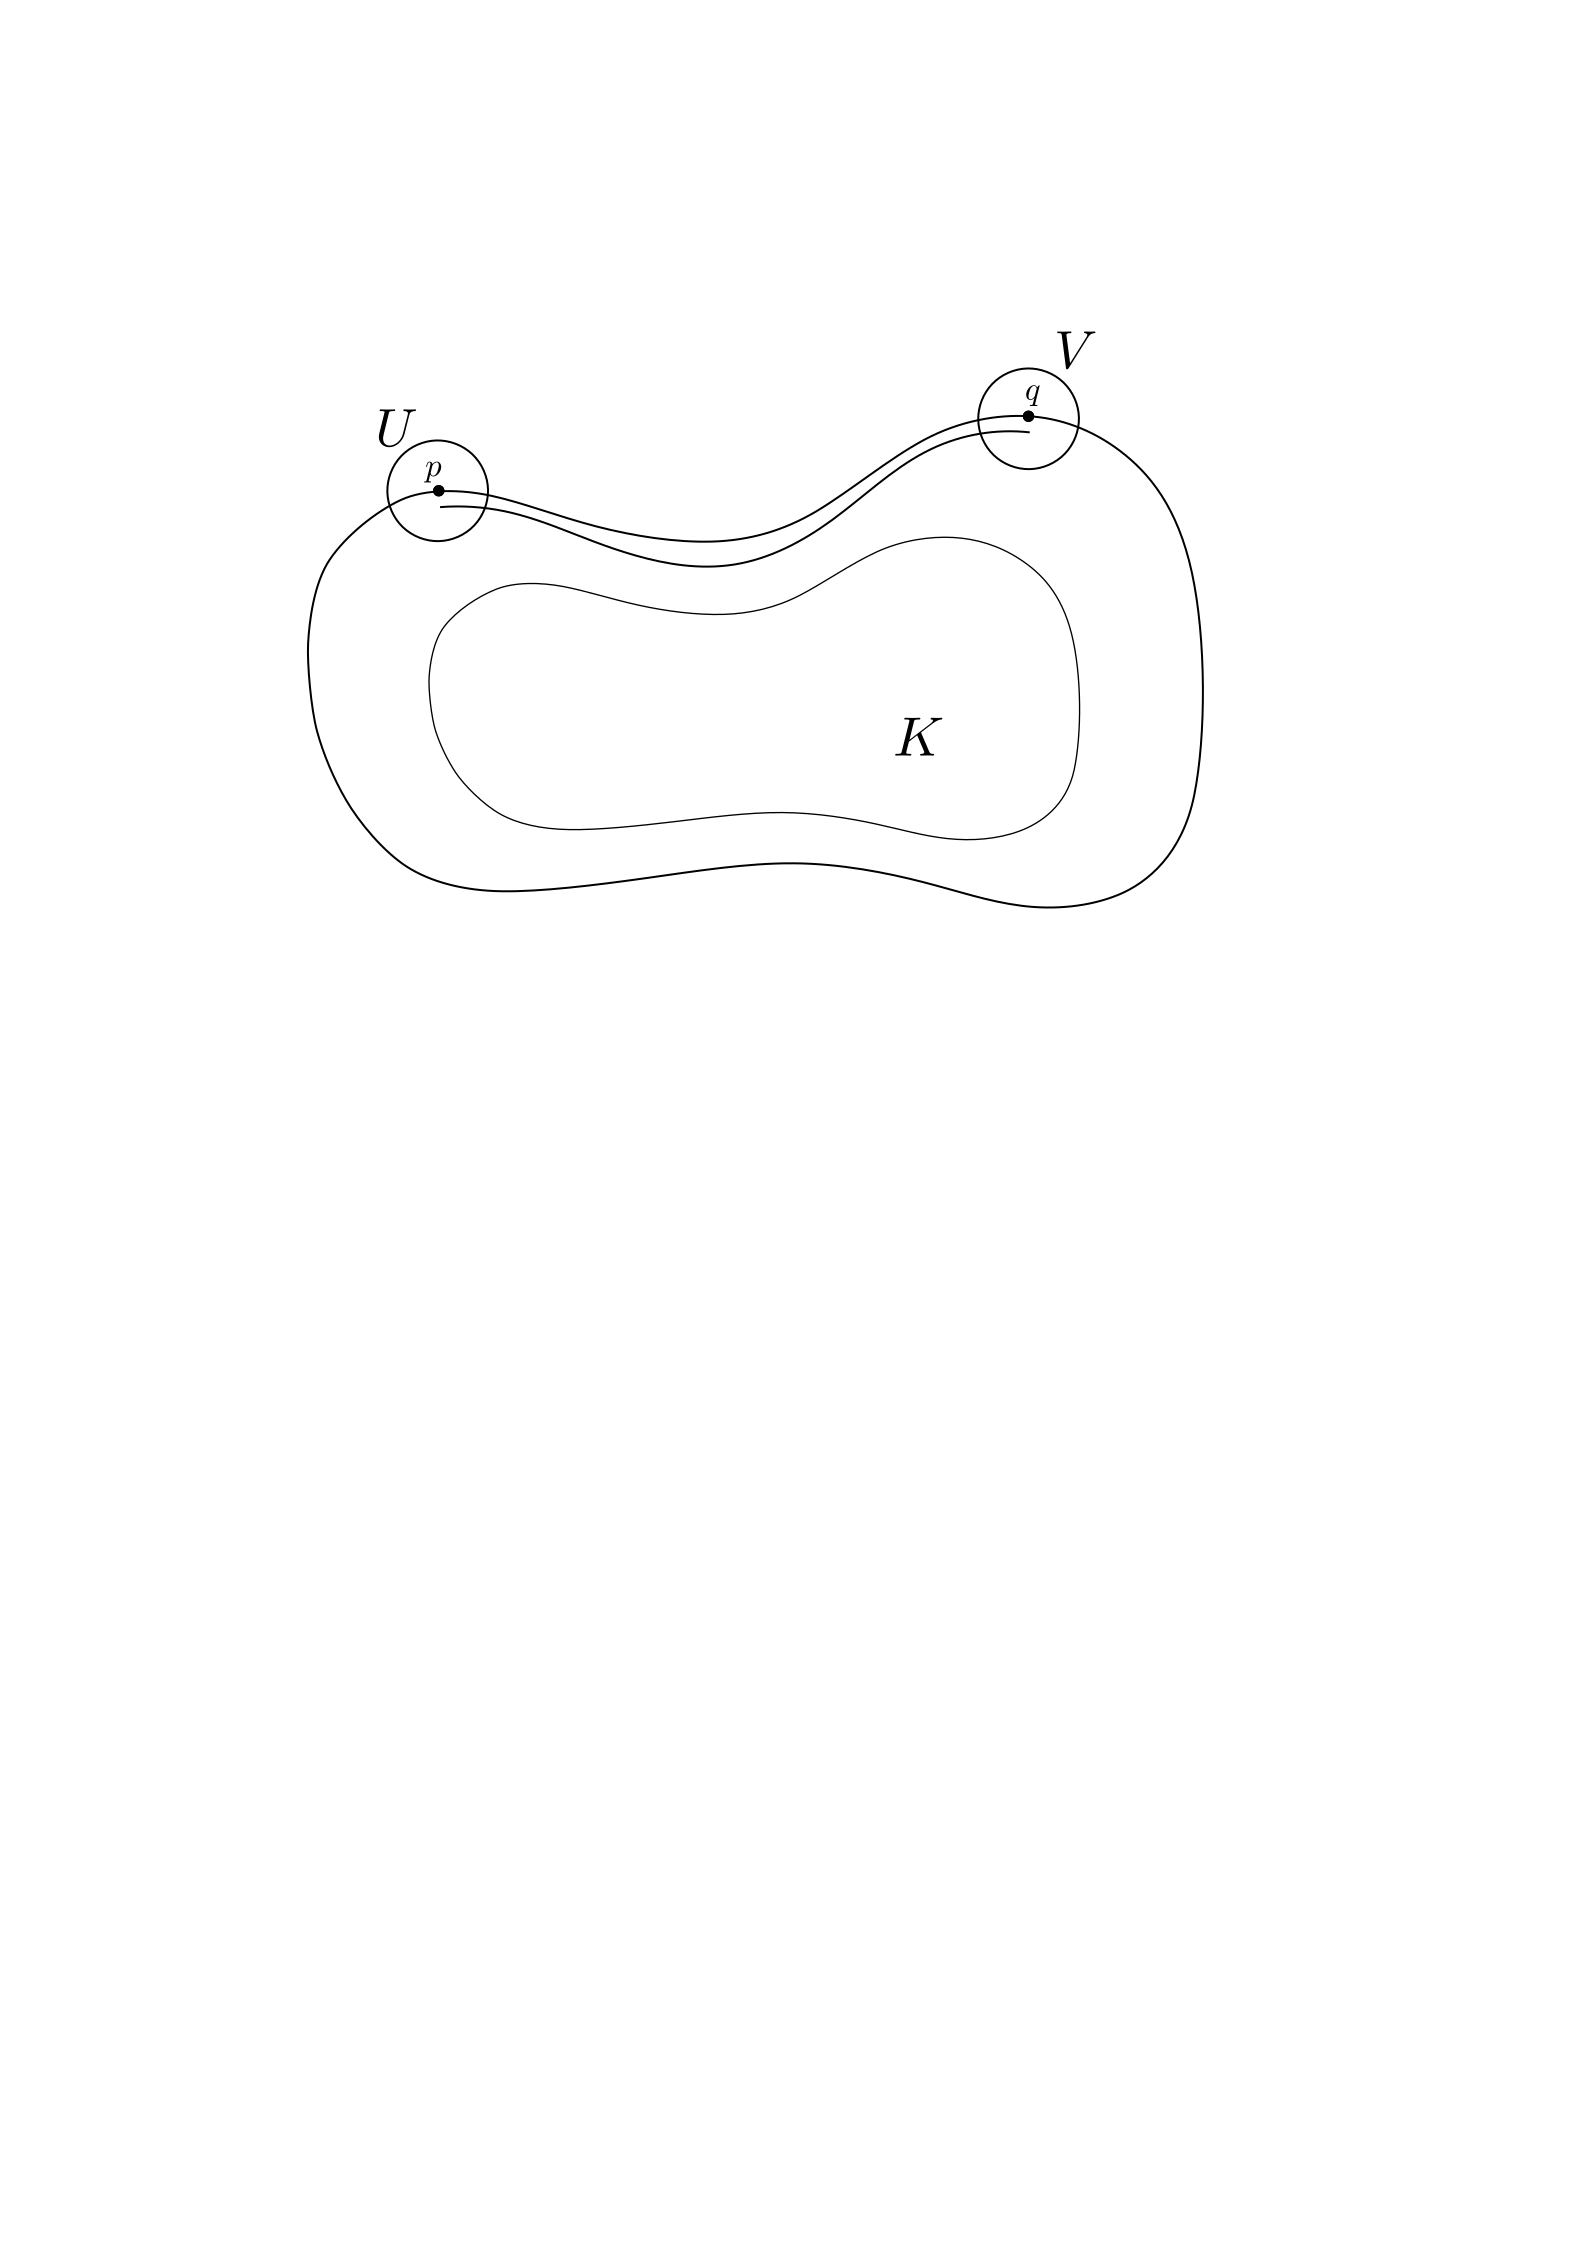
\includegraphics[width=1.05\textwidth, trim=0 18cm 0 3cm]{nonvis4.png}
  }
  \only<17>{
    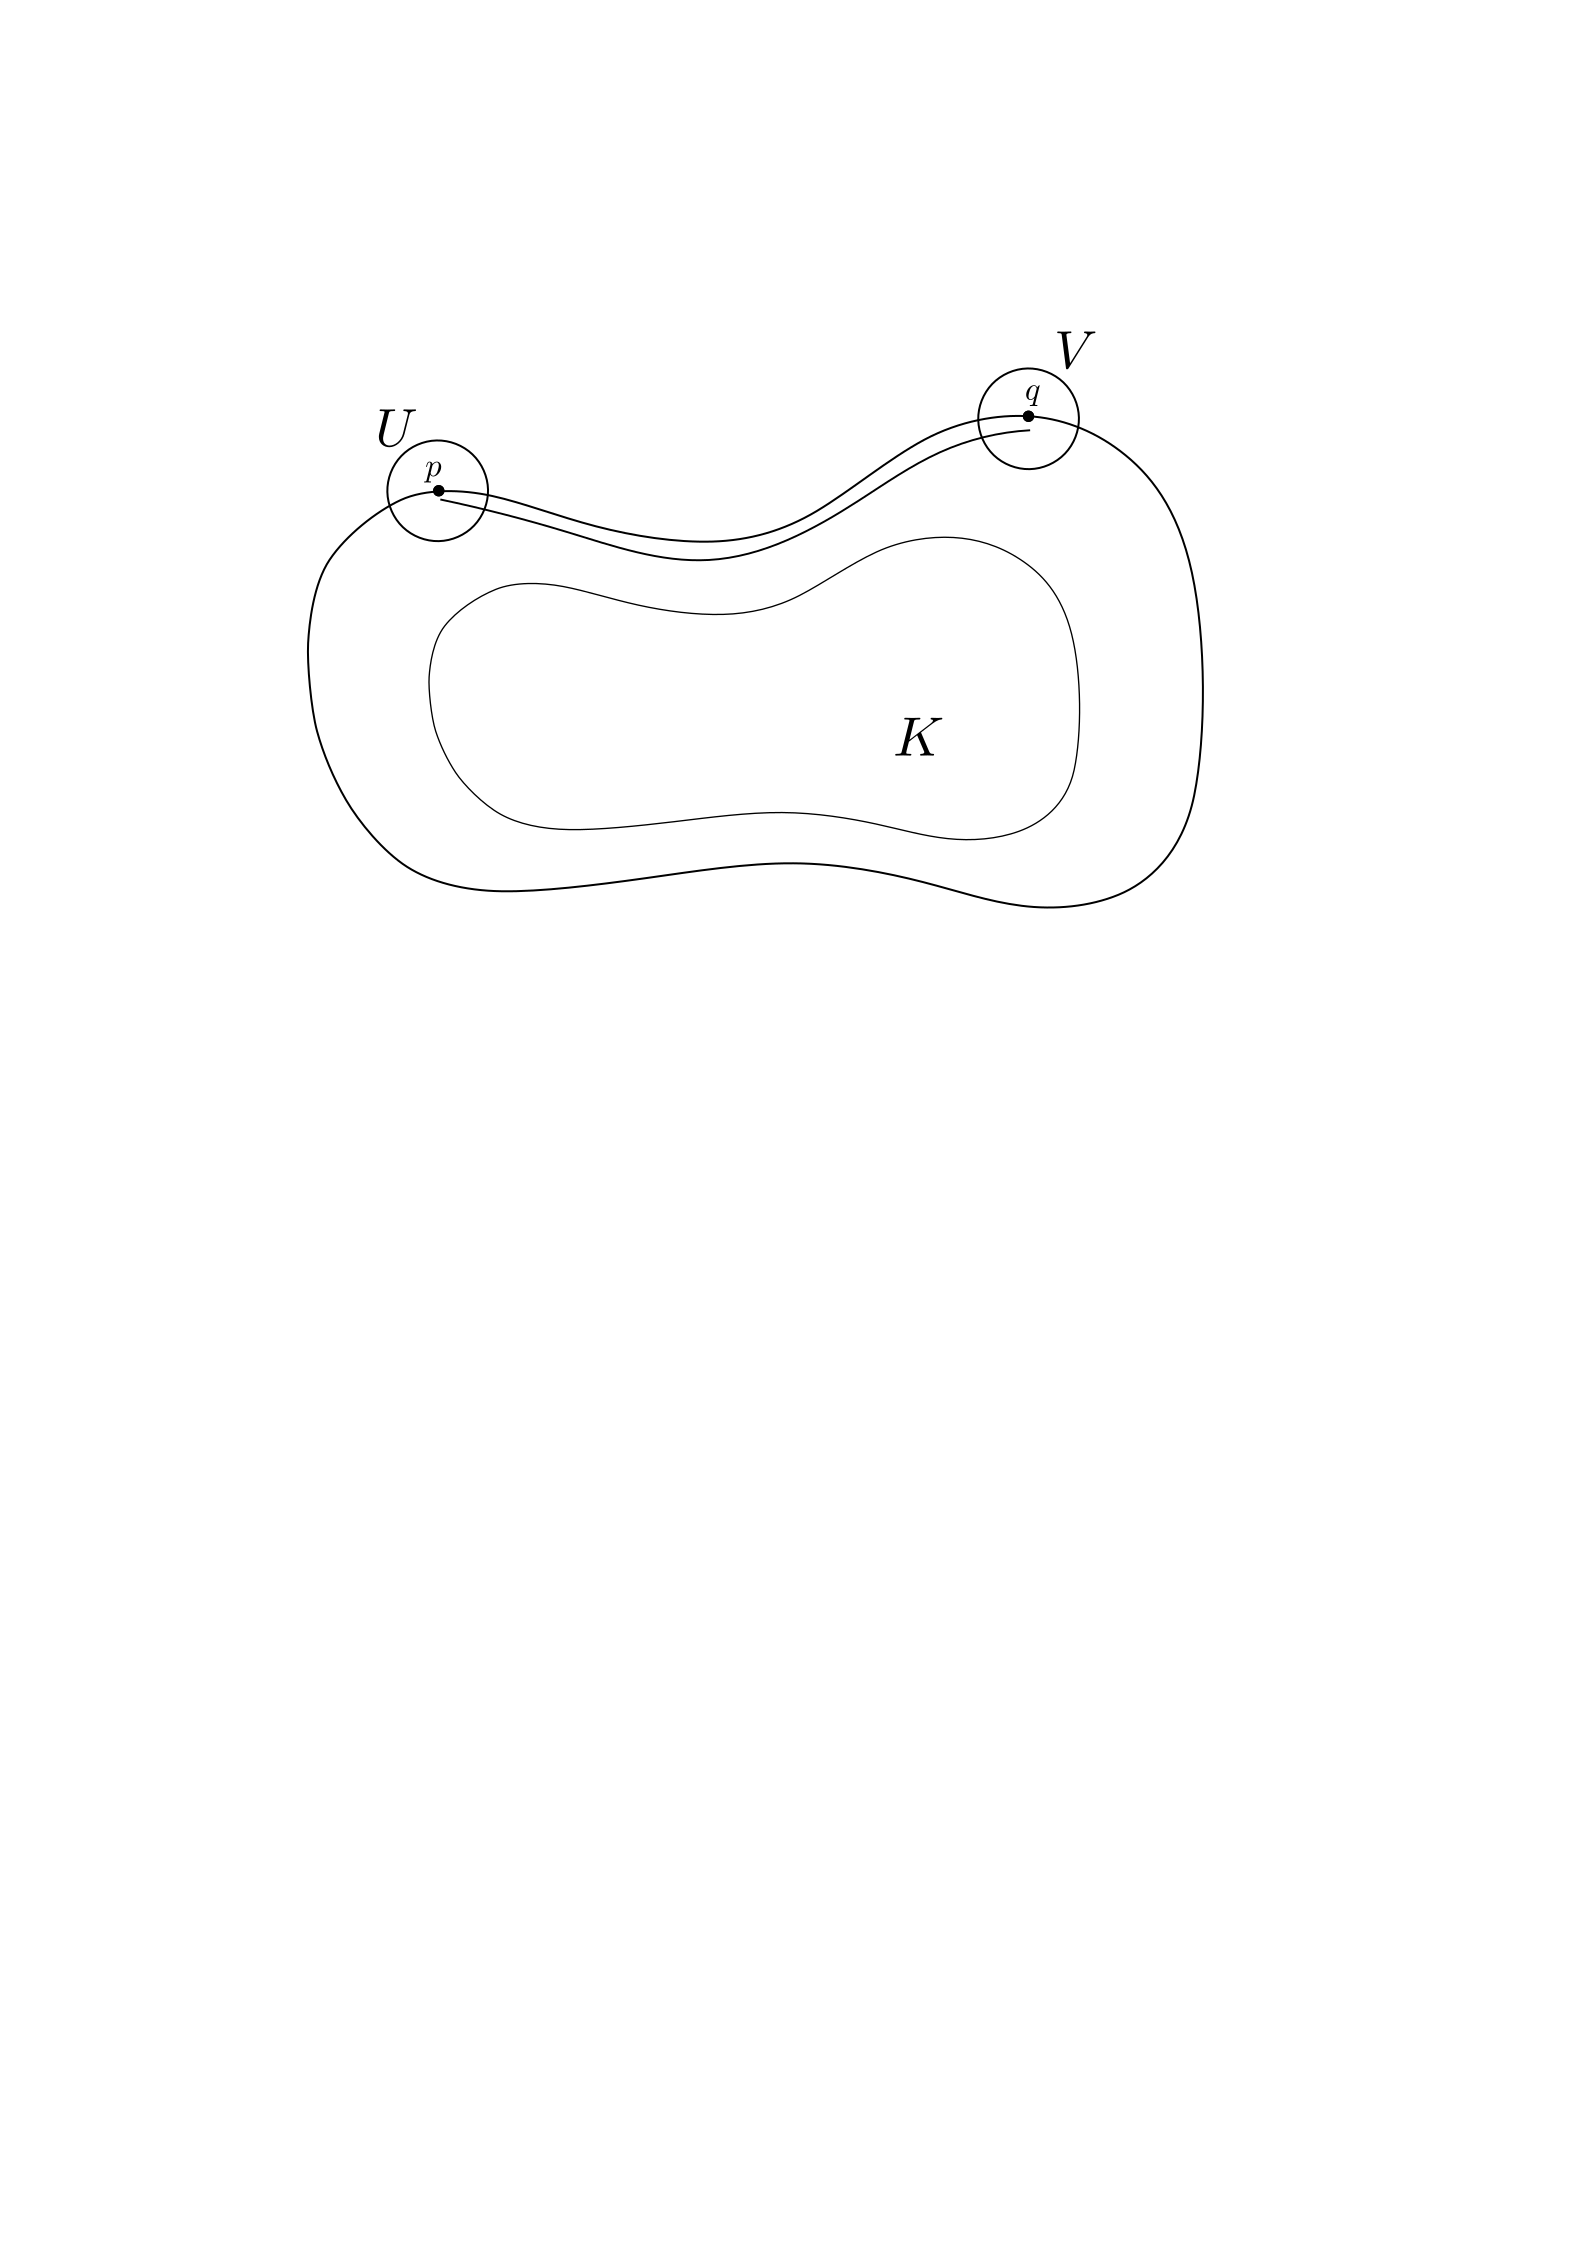
\includegraphics[width=1.05\textwidth, trim=0 18cm 0 3cm]{nonvis5.png}
  }
  \only<18>{
    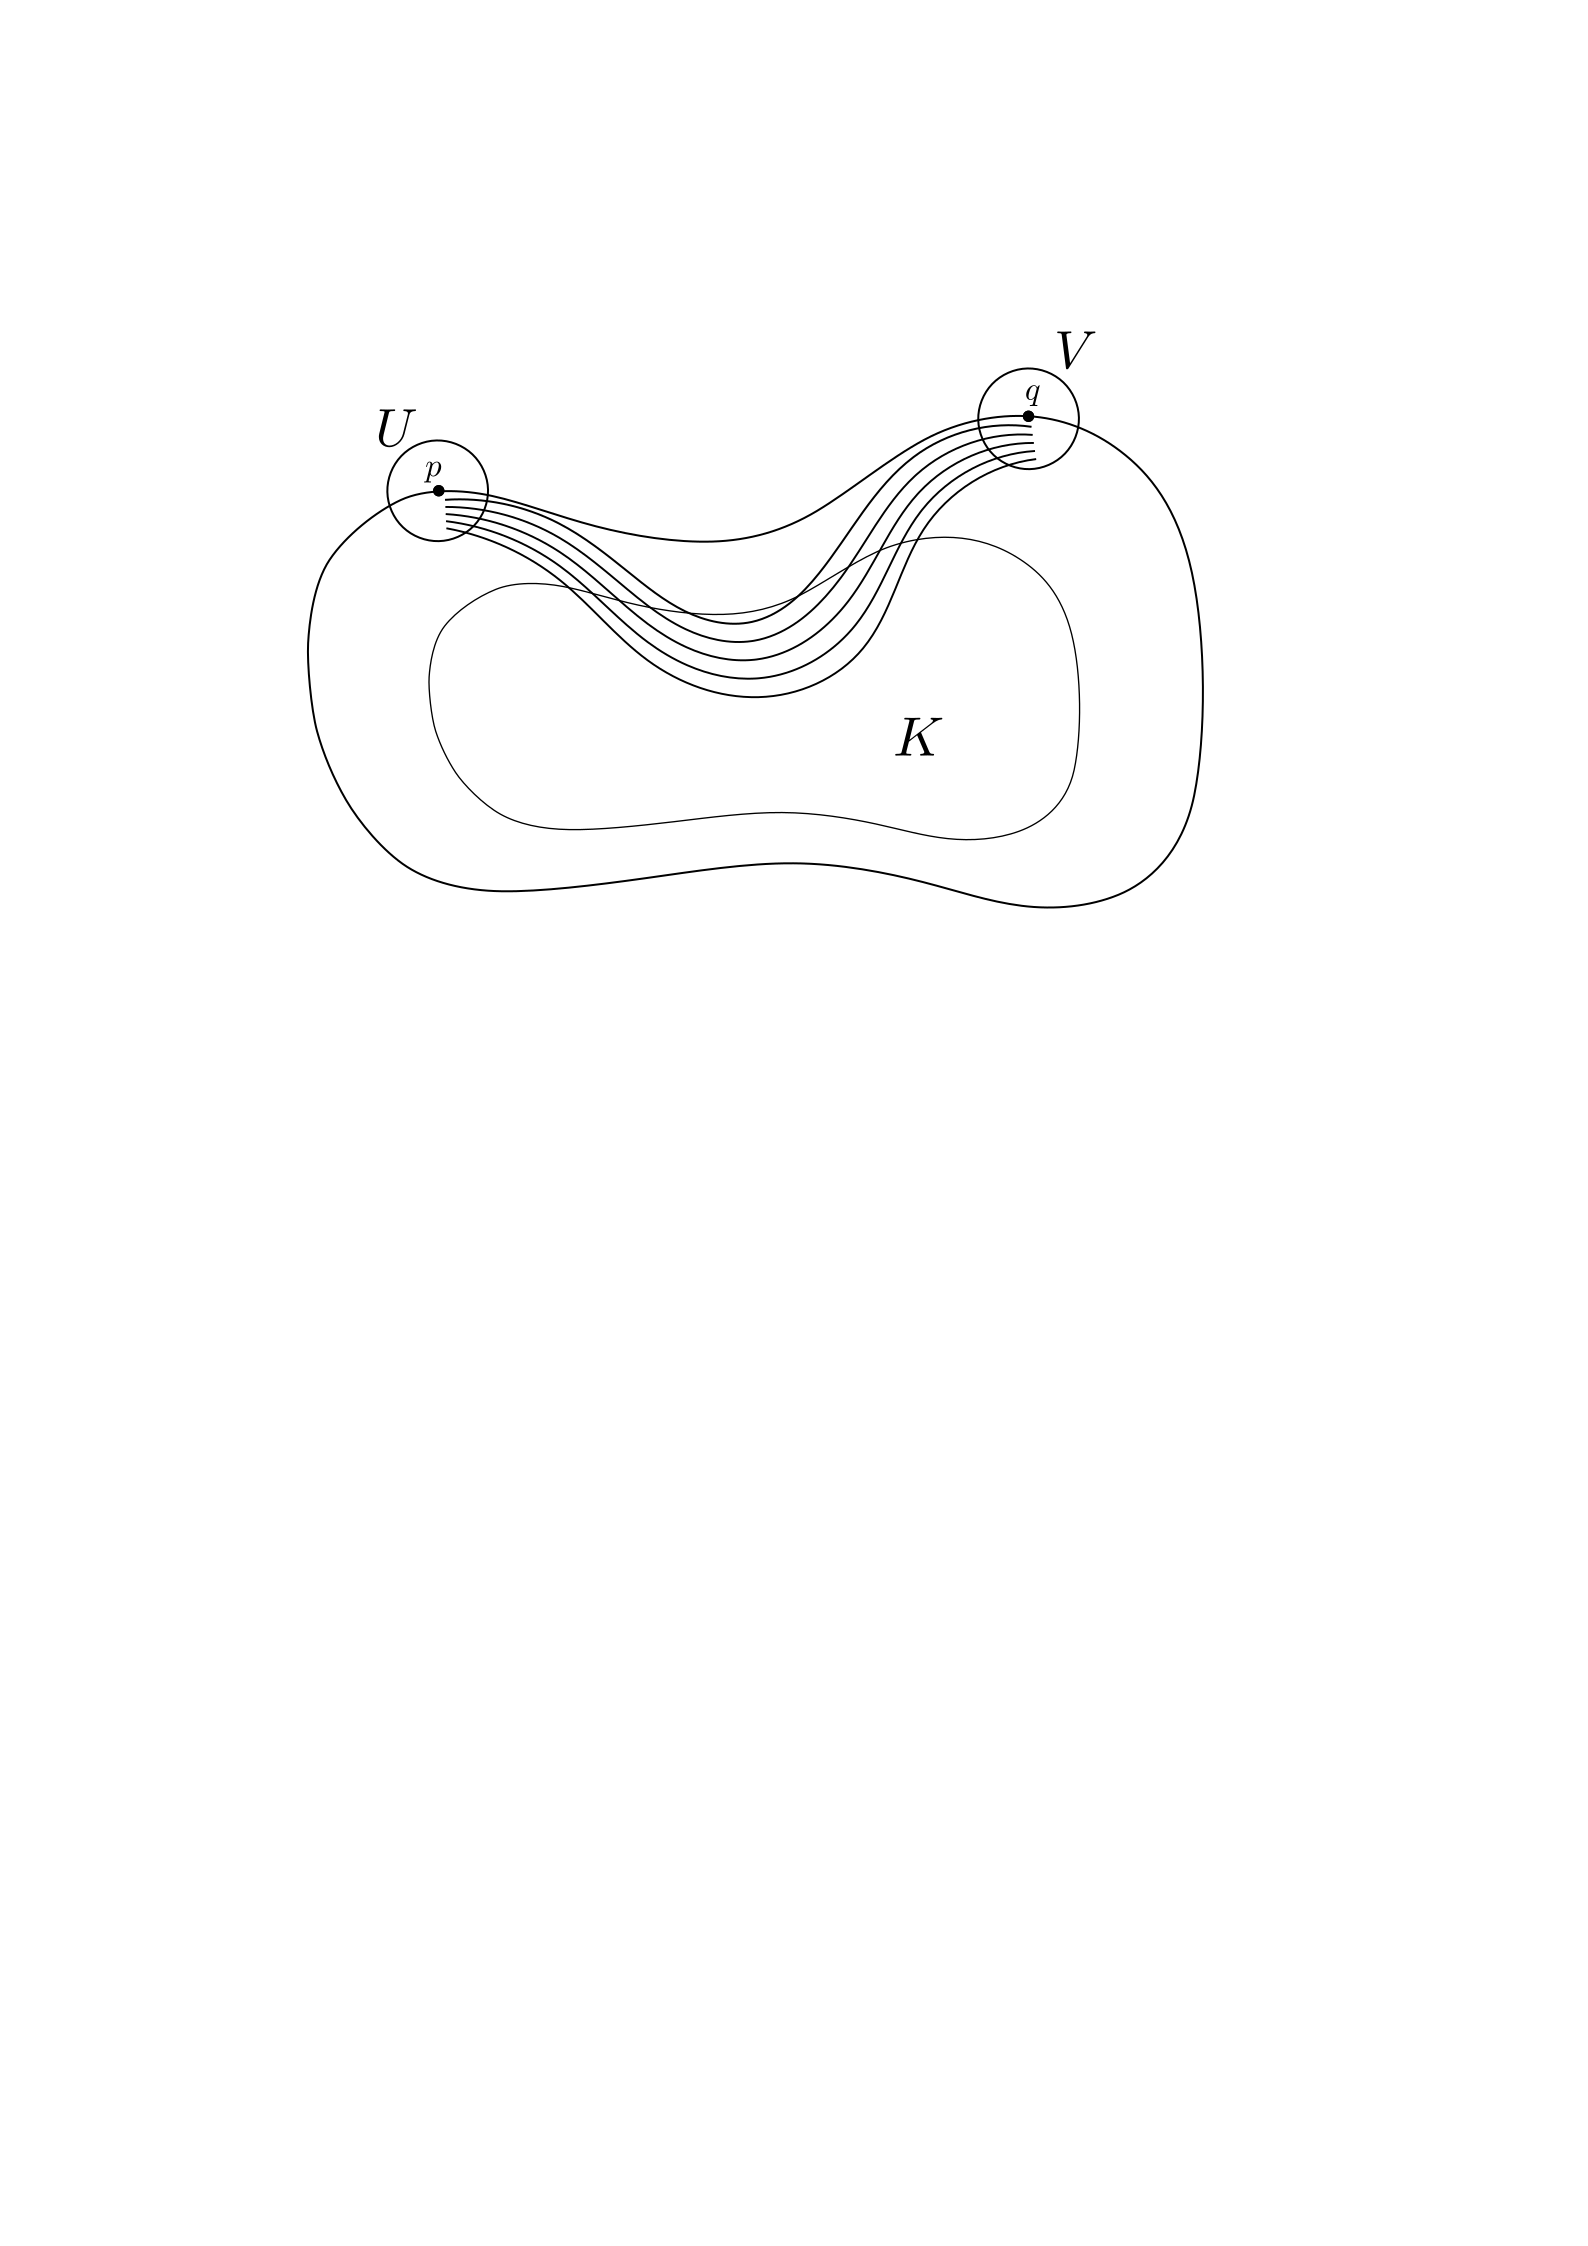
\includegraphics[width=1.05\textwidth, trim=0 16cm 0 3cm]{vis.png}
    Condizione di visibilità: le simil-geodetiche ``curvano verso l'interno'', rimanendo dentro il compatto $K$.
  }
\end{frame}